\section{PROFETA}
%------------------------------
\begin{frame}[label=3]{BDI Model}{Belief-Desire-Intention}  
\begin{itemize}
\item 
The BDI model is a philosophical theory of human reasoning 
   [\purple{Bratman et Israel}] that has been successfully applied to 
   \red{software agents} [\purple{Wooldridge, Jennings }] 
   \N
   \item
    In particular, we have:
    \begin{itemize}
      \n
      \item 
      \red{Beliefs}, that represent the \purple{knowledge} about both the world and 
      the state of the agent itself
      \n
      \item
      \red{Desires} (or \red{Goals}), that represent the \purple{objectives} the agent wants to achieve
      \n
      \item
      \red{Intentions}, the sequence of \purple{actions} that allows the agent to achieve a particular objective
    \end{itemize}



\end{itemize}
  \N\N
\end{frame}
%------------------------------

%------------------------------
\begin{frame}[label=5]{Agents}
  
  \begin{itemize}
  \pause
  \item
   \red{Agents} are entities that: 
  \begin{itemize}
    \item 
      \red{act} in a dynamic environment;
    \item
      \red{perceive} their surroundings through sensors;
    \item
      \red{adapt} their behaviour to respond to changes in the environment;
    \item
      \red{make} autonomous decisions to achieve its design goals;
    \end{itemize}
  \item
  \n
    The notion of agent is well suited to represent the behaviour of an AMR
  \end{itemize}

\end{frame}
%------------------------------





%
%%------------------------------
%%\subsection{}
%%------------------------------
%
%



















%
%\begin{frame}{Graph Models}
%  % Image
%  \begin{figure}[!h]
%    \begin{center}
%      \fbox{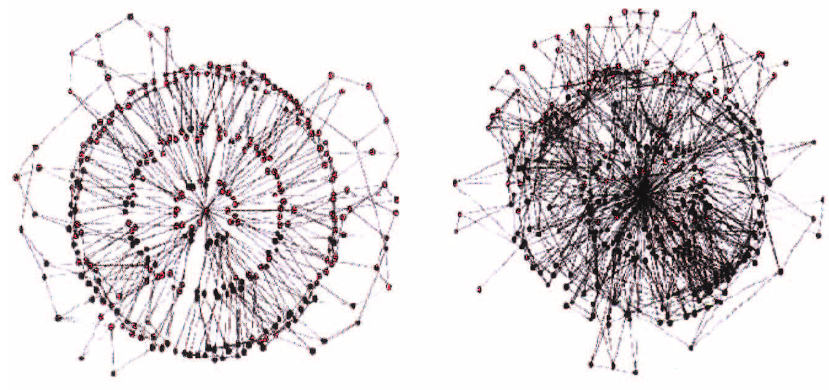
\includegraphics[width=150pt]{img/sample.png}}
%    \end{center}
%  \end{figure}
%\end{frame}
%%
%%
%\begin{frame}{Random Graphs}
%  \begin{itemize}
%    \item Formul\ae\\
%    \item \red{p}$*$\red{$N_1$}$*$(\red{N} - 1) / 2 connections
%  \end{itemize}
%\end{frame}
%%
%%
%\begin{frame}{SampleCode}
%We used the \red{peersim} library\footnote{\tiny{http://peersim.sourceforge.net/}} 
%  \begin{samplecode}
%    \begin{small}
%      // Generate a graph with an average of \red{k} connections\newline
%      // per node and randomness \red{r}\newline
%      Graph g = GraphFactory.wireKOut(g, k, r);\newline
%    \end{small}
%  \end{samplecode}
%\end{frame}
%%
%%
%\begin{frame}{SampleCode2}
%  \begin{samplecode}
%    \begin{tiny}
%      \begin{tabbing}
%        @WebService() \= public class \red{GraphService} \{\\
%        \> @WebMethod() public int [] \red{countNeighbours} (@WebParam() int [] adjVector) \{...\}\\
%        \> @WebMethod() public String [] \red{processConnections} (@WebParam() int [] neighboursCount) \{ ... \}\\
%        \> @WebMethod() \= public int [] \red{computeHops} ( @WebParam() int [] adjVector, \\
%        \> \> @WebParam() int [] neighbourCount,\\
%        \> \> @WebParam() int hyperNodeIndex) \{ ... \}\\
%        \}
%      \end{tabbing}
%    \end{tiny}
%  \end{samplecode}
%\end{frame}
%%
%
